\documentclass[conference]{IEEEtran}
\usepackage{graphicx}
\begin{document}

\title{Artificial Intelligence in Education: A Review}


\author{\IEEEauthorblockN{1\textsuperscript{st} Omkar Oak}
\IEEEauthorblockA{\textit{Dept. of Computer Engineering} \\
\textit{College of Engineering, Pune}\\
Pune, India \\
omkarsoak@gmail.com}
\and
\IEEEauthorblockN{2\textsuperscript{nd} Dr. Abhijit Joshi}
\IEEEauthorblockA{\textit{Dept. of Computer Engineering} \\
\textit{IIT, Bombay}\\
Mumbai, India \\
abhijitjoshi@iitb.edu.in}
\and
\IEEEauthorblockN{3\textsuperscript{rd} Prof. Manoj Kumar}
\IEEEauthorblockA{\textit{Dept. of Computer Engineering} \\
\textit{College of Engineering, Pune)}\\
Pune, India \\
kumaarmanoj@coep.ac.in}
}

\maketitle

\begin{abstract}
Artificial intelligence is a field of study and the resulting innovations and developments that have culminated in computers, machines, and other artifacts having human-like intelligence characterized by cognitive abilities, learning, adaptability, and decision-making capabilities. The study ascertained that AI has extensively been adopted and used in education, particularly by education institutions, in different forms. AI initially took the form of computer and computer related technologies, transitioning to web-based and online intelligent education systems, and ultimately with the use of embedded computer systems, together with other technologies, the use of humanoid robots and web-based chatbots to perform instructors' duties and functions independently or with instructors.
\end{abstract}
\vspace{3 mm}
\begin{IEEEkeywords}
learning quality,machine learning,teaching activities,student assignments grading,Web-based chatbots,
\end{IEEEkeywords}

\section{Introduction}
Prior to the introduction of computers and other related technologies, instructors and students, engaged in instructions and learning mechanically, or through the pure application of natural human effort. With the introduction of microcomputers, and by extension, personal computers in the 1970s, which according to Flamm, provided more computing power and marked an important transition to electronic computers for the mass market [1]. In agreement, Campbell-Kelly opined that with developments of the electronic computers, more particularly, and the availability of the same for different entities across different sectors of the economy, was precipitated by the developments of personal computers in the 1970s [2]. Personal computers development made it possible for individuals and other non-governmental entities to own and use computers for different reasons. These transitions harbingered the proliferation of computers in different sectors of the economy and society.

\section{Ease of Use}

\subsection{Artificial Intelligence in Current Education}
The mention of artificial intelligence brings to mind a supercomputer, a computer with immense processing capabilities, including adaptive behavior, such as inclusion of sensors, and other capabilities, that enable it to have human-like cognition and functional abilities, and indeed, which improve the supercomputers interaction with human beings.
\section{Purpose of the Study}
With the continued application or use of information technology, it is inevitable that it has impacted the education in different ways. This study seeks to assess how the use of AI, in its different forms, in education, has impacted or affected different aspects of education. More particularly, the study will seek to assess how AI has affected teaching, learning, and administration and management areas of education.

\subsection{Review Strategy}\label{AA}
The study seeks to assess the impact of AI on education. More particularly, it seeks to ascertain how AI has affected education, looking at various aspects of education, including administration, instruction, and learning. Accordingly, the study takes a retrogressive approach, entailing assessing secondary data and materials or studies that have been undertaken. Indeed, Snyder posited that a systematic or semi-systematic literature review, a review of secondary data, provides a deeper understanding of the study phenomenon \cite{b1}.
\vspace{-5mm}
\begin{center}
\begin{figure}[h]
\caption{Papers in AI/ML in the last 10 years}
\vspace{5 mm}
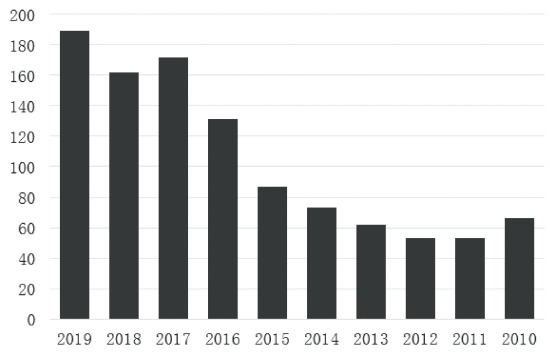
\includegraphics[width=9 cm]{graph1}
\end{figure}
\end{center}

\subsection{Search Strategy}
\begin{itemize}
\item Key words and search strings will be used to search different databases, including EBSCOhost, ProQuest,Web of Science.
\item In addition, the key words and search strings are used to search Google Scholar to identify articles from different journals that have focused on researching the impact of AI on education.
\item The journals containing the articles are then searched on Scimago and the journals with an H-Index of 20 and above are included in the study.
\item An H-Index is an author level measure of scientific productivity in terms of publications and citations and by extension, contribution to science and scholarly pursuits; and the higher the H-Index, the more reputable the journal and the authors published in the journal are.
\end{itemize}

\subsection{Sampling: Exclusion and Inclusion Criteria}
Initially, a total of 250 articles, published after 2009 were selected premised on the aforementioned criteria; matching the search key words and search strings and inclusion in a journal with an H-Index of 20 and above. A further review and analysis of these articles, identifying articles that focused on the nature of AI and the impact it had on education, together with the H-Index, narrowing down the number of articles for analysis to thirty, a sample size that was considered sufficient to inform conclusions and inferences about the impact of AI on education, taking a retrospective approach. 

\subsection{Machine Learning}

The core of machine learning is knowledge discovery, the process of parsing based on sampling data set known as “training data”, generating meaningful patterns and a structured knowledge. For instance, machine learning can help create recommendations for students as they select classes, even choose universities. It leverages achievements data, aspirations, preferences of students to “match-make” institutions where they can be best developed. Moreover, this technology can help instructors gain an understanding of how every concept is being digested by students [4]. \\
\vspace{-6mm}
\begin{table}[h]
\begin{center}
\caption{Neural Networks}
\begin{tabular}{|c|c|}
\hline
\textbf{Neural Network Parameters} & \textbf{Ranges} \\ \hline
Number of inputs  & 3 \\ \hline
Number of outputs & 1 \\ \hline
Number of neurons & 15\\ \hline
Training Algorithm & Lavenberg Marquadt\\ \hline
Layer transfer function & Tan-sigmoidal \\ \hline
Learning Rate & 0.12\\ \hline
Testing Ratio & 0.7\\ \hline
\end{tabular}
\end{center}
\end{table}

In particular, for student assessment, image recognition and prediction of machine learning can be used to grade student assignments and exams, with faster and more reliable results than human being. It should be noted that deep learning, the subfield of machine learning, attracts much attention. This widely used techniques includes decision tree learning, inductive logic programming, clustering, reinforcement learning and Bayesian networks. \\
From technique perspective, deep learning emphasizes on increasingly meaningful representations from learning successive layers. These layer features are extracted via models called neural networks structured in literal layers stacked on top of each other.

\subsection{AI in Learning}
\begin{itemize}
\item Learning, which is an integral part of education, is another aspect of education that is within the scope of the study. 
\item From an evaluation and analysis of the different articles included in the study, different ways in which AI has been adopted and implemented or leveraged in fostering students’ learning were identified.
\vspace{-3 mm}
\begin{center}
\begin{figure}[h]
\caption{Technological structure of AI Education}
\vspace{5 mm}
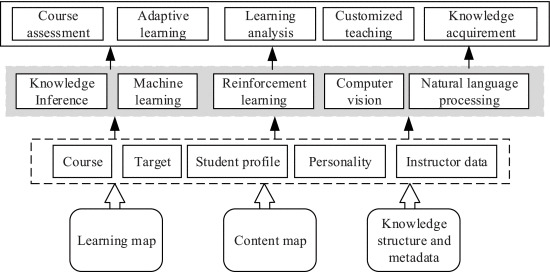
\includegraphics[width=9 cm]{graph2}
\end{figure}
\end{center}
\vspace{-3 mm}
\item Further, specific programs or applications that leverage AI to improve student learning were identified. An important way in which AI has been applied in improving students’ learning is the customization and personalization of curriculum and content in line with the learners needs, abilities, and capabilities \cite{b3}.
\item On the other hand, as gleaned from other articles, there were other applications of AI that were found to have a major impact on the learners’ experiences. 
\item AI learning is currently considered as education assistant at the early stage, while AI-enable education will play a more important role as learning requirements changes. 
\item It now provides courses of different difficulty based on simple rule judgement and has not reached the best intelligence level in intelligent education. 
\item There are education studies for AI systems involving knowledge map and probability model\cite{b2}.
\end{itemize}


\begin{thebibliography}{00}
\bibitem{b1} G. Eason, B. Noble, and I. N. Sneddon, ``On certain integrals of Lipschitz-Hankel type involving products of Bessel functions,'' Phil. Trans. Roy. Soc. London, vol. A247, pp. 529--551, April 1955.
\bibitem{b2} “Theory of computer science”, E. V. Krishnamurthy, 2004, Affiliated East Press Publications, ISBN-10: 038791255X / ISBN-13: 978-0387912554. 
\bibitem{b3} I. S. Jacobs and C. P. Bean, ``Fine particles, thin films and exchange anisotropy,'' in Magnetism, vol. III, G. T. Rado and H. Suhl, Eds. New York: Academic, 1963, pp. 271--350.
\bibitem{b4} “Elements of the Theory of Computation”, Harry Lewis, Christos H. Papadimitriou, 2nd Edition, 1997, Prentice-Hall Publications, ISSN 0891-4516.
\bibitem{b5} “Advanced MSDOS Programming”, Ray Dunkon, 2nd Edition, BPB Publication, ISBN 1- 55615-157-8
\end{thebibliography}
\end{document}